% 
% Annual Cognitive Science Conference
% Sample LaTeX Paper -- Proceedings Format
% 

% Original : Ashwin Ram (ashwin@cc.gatech.edu)       04/01/1994
% Modified : Johanna Moore (jmoore@cs.pitt.edu)      03/17/1995
% Modified : David Noelle (noelle@ucsd.edu)          03/15/1996
% Modified : Pat Langley (langley@cs.stanford.edu)   01/26/1997
% Latex2e corrections by Ramin Charles Nakisa        01/28/1997 
% Modified : Tina Eliassi-Rad (eliassi@cs.wisc.edu)  01/31/1998
% Modified : Trisha Yannuzzi (trisha@ircs.upenn.edu) 12/28/1999 (in process)
% Modified : Mary Ellen Foster (M.E.Foster@ed.ac.uk) 12/11/2000
% Modified : Ken Forbus                              01/23/2004
% Modified : Eli M. Silk (esilk@pitt.edu)            05/24/2005
% Modified : Niels Taatgen (taatgen@cmu.edu)         10/24/2006
% Modified : David Noelle (dnoelle@ucmerced.edu)     11/19/2014
% Modified : Roger Levy (rplevy@mit.edu)             12/31/2018



%% Change "letterpaper" in the following line to "a4paper" if you must.

\documentclass[10pt,letterpaper]{article}

\usepackage{cogsci}

\cogscifinalcopy % Uncomment this line for the final submission 


\usepackage{pslatex}
\usepackage{apacite}
\usepackage{float} % Roger Levy added this and changed figure/table
                   % placement to [H] for conformity to Word template,
                   % though floating tables and figures to top is
                   % still generally recommended!
                   
\usepackage{ifxetex,ifluatex}
\usepackage{microtype}
\makeatletter
\makeatother
\usepackage{xcolor}
\usepackage{xurl}
\usepackage{amsmath} % keep the package, plz

\urlstyle{same} % disable monospaced font for URLs
\usepackage{graphicx}
\usepackage{wrapfig}
\makeatletter
\def\maxwidth{\ifdim\Gin@nat@width>\linewidth\linewidth\else\Gin@nat@width\fi}
\def\maxheight{\ifdim\Gin@nat@height>\textheight\textheight\else\Gin@nat@height\fi}
\makeatother
\setkeys{Gin}{width=\maxwidth,height=\maxheight,keepaspectratio}
% Set default figure placement to htbp
\makeatletter
\def\fps@figure{htbp}
\makeatother
\setlength{\emergencystretch}{3em} % prevent overfull lines
\providecommand{\tightlist}{%
  \setlength{\itemsep}{0pt}\setlength{\parskip}{0pt}}
\setcounter{secnumdepth}{-\maxdimen} % remove section numbering
\ifluatex
  \usepackage{selnolig}  % disable illegal ligatures
\fi

%\usepackage[none]{hyphenat} % Sometimes it can be useful to turn off
%hyphenation for purposes such as spell checking of the resulting
%PDF.  Uncomment this block to turn off hyphenation.

%\setlength\titlebox{4.5cm}
% You can expand the titlebox if you need extra space
% to show all the authors. Please do not make the titlebox
% smaller than 4.5cm (the original size).
%%If you do, we reserve the right to require you to change it back in
%%the camera-ready version, which could interfere with the timely
%%appearance of your paper in the Proceedings.


\title{Statistical Power in Response Signal Paradigm Experiments}
 
\author{{\large \bf Pavel Logačev (pavel.logacev@boun.edu.tr)} \\
  Boğaziçi University, Department of Linguistics \\
  34342 Beşiktaş, İstanbul
  \AND {\large \bf M. İlteriş Bozkurt (ilteris.bozkurt@metu.edu.tr)} \\
  Middle East Technical University, Cognitive Science Department \\
  06800 Çankaya, Ankara}


\begin{document}


\maketitle

\begin{abstract}
The speed-accuracy tradeoff (SAT) method has produced several prominent findings in sentence processing. While a substantial number of SAT studies have yielded statistical null-results regarding the degree to which certain factors influence the speed of sentence processing operations, the statistical power of the SAT paradigm is not known. As a result, it is not entirely clear how to interpret these findings.
We addressed this problem by means of a simulation study in which we simulated SAT experiments for a range of known effect sizes in order to determine the statistical power in typical SAT experiments.
We found that while SAT experiments appear to have quite satisfactory power to detect differences in asymptotic accuracy, that is not the case for speed-related parameters, especially for the multiple-response variant of the technique. We conclude that the failure to find an effect in speed-related parameters in SAT experiments may be less meaningful than previously thought.

\textbf{Keywords:} 
response signal paradigm; speed-accuracy tradeoff; statistical power; simulation
\end{abstract}

\section{Introduction}\label{introduction}

Experimental paradigms for measuring the speed-accuracy tradeoffs in cognitive tasks have been essential in many areas of cognitive science \cite<e.g.,>[]{Heitz2014} because they address a potentially problematic aspect of typical reaction time (RT) tasks: Most cognitive tasks can be performed more accurately at the cost of lower speed, or faster at the expense of accuracy (e.g., \citeNP{Pachella1974}). As a result, the average RT and accuracy obtained in such tasks reflect not only the processing speed and accuracy on that task, but also the participant's \textit{response criterion}, i.e., the mechanism by which they determine that they have processed a stimulus to a sufficient degree to respond. 
\textit{Speed-accuracy tradeoff functions (SATFs)}, which describe the increase in response accuracy over time, are unaffected by the participants' response criteria and thus offer a way to obtain uncontaminated estimates of the relative speed of mental processes separately from their ultimate probabilities of success.

Differences between the SATFs can yield important insights into the timing of cognitive processes and have been successfully used in areas as diverse as attention, vision, memory, and psycholinguistics. 
%
%For example, \citeA{Carrasco2001} used the % response signal, because we have it as a section later
%SAT procedure in two visual search tasks. They demonstrated that in a simple \textit{feature search} task, the number of distractors of another orientation as well as cueing of the target location did not affect the processing time, but only the maximally attainable degree of discriminability (\textit{asymptotic discriminability}). Importantly, this was not the case in a \textit{conjuction search} task, in which participants searched for a unique combination of two features like orientation and spatial frequency among distractors that shared only one of them: Set size and cueing of the target location affected both, asymptotic discriminability as well as processing time. 
% Taken together, their results suggest that the allocation of covert attention affects discriminability and the rate of information processing.
%
%(e.g., searching for a target of one orientation among distracters of another orientation) and \textit{conjunction search} (e.g., searching for a unique combination of two features like orientation and spatial frequency among distracters that share only one of them). 
%
%According to their results, as set size increased in feature search, asymptotic discriminability decreased and processing time was not affected when target location was not cued, and discriminability increased but processing time remained unaffected when target location was \textit{cued}; as set size increased in conjunction search, asymptotic discriminability decreased and processing time was affected when target location was not cued, and discriminability increased and processing time was affected when target location was \textit{cued}. In the end, their use of the response signal paradigm to control for SATs enabled them to show that covert attention improves discriminability and the rate of information processing.
%(see also \citeNP{Carrasco2004} for a follow-up on the existence of \textit{temporal performance fields} and how covert attention affects them, \citeNP{Liu2009a} for an investigation of the \textit{mask-dependent cuing effect}, \citeNP{Mihaylova2010} for a comparison of detection speeds of illusory vs. real images, \citeNP{Zhao2011} on how \textit{inhibition of return} is related to criterion shifts and processing delays, \citeNP{Kobayashi2020} on how facilitation by contextual memory arises very early in visual search process).
% Two back-to-back examples that start with "For example": Liu2009a and McElree2000, maybe we can express in some way that the McElree one is the sentence processing one.
% We can add Ratcliff (2008), two Öztekins (2009), and some others that do not exactly use SAT as the experimental paradigm we focus on, and Heitz (2014) for a review for such papers.
% Reed1973,McElree1993
%involving the processing of sentences or other stimuli, speed and accuracy are related, 
% ... accuracy is never perfect and so we can't know that the RT is the processing time ...
%
%In another SAT study, 
For example, \citeA{McElree2000} showed that in the resolution of filler-gap dependencies in sentences like (1), increased distance between the verb \textit{'admired'} and the head noun of its subject (\textit{'book'}) decreased the \textit{probability of successful dependency resolution}, but had no effect on the \textit{processing speed}. That is, while participants did quite well at correctly judging grammatical sentences like (1a) and their ungrammatical counterparts like (1a') after a sufficient amount of time, they did not perform as well with sentences like (1b) and (1b'). However, the speed of relative increase in accuracy was the same in both condition pairs. Because discriminating between grammatical and ungrammatical sentences in (1) arguably requires the retrieval of \textit{book} from working memory, this finding suggests that in sentence comprehension, distance affects the probability of successful retrieval of dependents from memory, but not the speed of the retrieval process.

\setlength{\leftmargini}{3.2em}
\begin{itemize}
\item[(1a/a')] This was the \textit{book} that the editor \textit{admired/*amused}. 
\item[(1b/b')] This was the \textit{book} that the editor who the receptionist married \textit{admired/*amused}.
\end{itemize}

This finding, as well as a number of other results in the SAT literature  \cite<e.g.,>[among many others]{Foraker2007,Martin2008,McElree2003,VanDyke2011} rest on the absence of a significant difference in speed-related parameters of the speed-accuracy tradeoff function. Because SAT data analysis typically involves numerical estimation of several parameters describing the SATF in each condition, followed by a variant of a \textit{stepwise model selection procedure} \cite<e.g.,>{Thompson1978}, it is unfortunately not clear how much statistical power such experiments have in order to find differences in processing speed (however, see \citeNP{Pankratz2021}, who conducted a power analysis using data from \citeNP{Franck2020}, a published SAT study, and showed a lack of statistical power).
In order to understand how to interpret such statistical null-results, we conducted a simulation study to determine the amount of statistical power in typical SAT experiments.

% todo
Importantly, although our simulations are meant to model SAT experiments typical for the area of sentence processing, our results will likely be relevant beyond this specific setting. We further 
make all code available online,\footnote{\url{https://git.io/JsfPR}} which allows anyone to re-run the power simulations presented here under different assumptions with a modest amount of effort.


\section{The Response Signal Paradigm}\label{the-response-signal-paradigm}

A method commonly used to estimate SATFs is the \textit{response-signal paradigm} (\citeNP{McElree1993,Reed1973}). In this paradigm, participants see stimuli of different types 
% (e.g., sentences like (1)).
and are asked to respond to them after varying amounts of time relative to the onset of the last phrase of the sentence.
% In sentence processing experiments, sentences are presented phrase by phrase, and participants judge their acceptability.
Typically, an auditory cue presented after a variable amount of time is used as cue to respond immediately, even if participants have not yet finished making a decision. In the so-called \textit{single-response} variant (\textit{SR-SAT}), participants are prompted to respond once per trial. In the \textit{multiple-response} variant (\textit{MR-SAT}), participants respond several times per trial, at different lags.

As in the \citeA{McElree2000} experiment, the experimental design needs to ensure that discrimination between different types of stimuli (such as \textit{`acceptable'} and \textit{`unacceptable'}) requires participants to deploy the cognitive process being studied. As a result, the difference between SATFs (at least partially) reflects the timing of the cognitive process involved -- the number of trials on which the relevant process has terminated will increase with the passage of time, and so will accuracy for both types of stimuli. In keeping with \textit{Signal Detection Theory (SDT)} terminology \cite{Wickens2001}, we will refer to the two types of stimuli as \textit{signal} and \textit{noise} without loss of generality.

In order to obtain estimates of sensitivity to stimulus type which is unaffected by response bias towards either response, the accuracy at each lag in each experimental condition pair is computed as the SDT sensitivity measure $d' = \Phi(\textit{hits}) - \Phi(\textit{false alarms})$, where $\Phi$ is the Gaussian distribution function, and \textit{hits} and \textit{false alarms} are the proportions of `signal' responses in signal and noise conditions, respectively. The resulting $d'$ values at each lag allow us to estimate the underlying SATF in each experimental condition, which is typically well-approximated by the negatively accelerated shifted exponential function in equation \ref{eq:satf} \cite{Dosher1979} which is illustrated in Figure \ref{fig:illustrationSATF}. In it, $\lambda$ (\textit{asymptotic accuracy}) determines the highest attainable level of accuracy given unlimited processing time, while $\delta$ (\textit{intercept}) and $\beta$ (\textit{rate}) jointly determine the processing speed: $\delta$ determines at which point the accuracy rises above chance, while $\beta$ determines how quickly the SATF increases. The reciprocal of the rate $\beta^{-1}$ can be interpreted as the time required for the function to reach approximately $63\%$ of the asymptote, \textit{once accuracy has departed from $0$}.
A joint measure of dynamics, $(\delta+\beta^{-1})$, can be interpreted as the time requires to reache $63\%$ of the asymptote, \textit{starting at 0} (e.g., \citeNP{Foraker2018,Liu2009b}). 


\vspace{-0.3cm}
\begin{equation}
d_t' = \lambda \cdot \left(1-e^{-\beta(t-\delta)} \right),~for~t > \delta;~else~d_t'=0
\label{eq:satf}
\end{equation}

\begin{figure}[t]
\centering
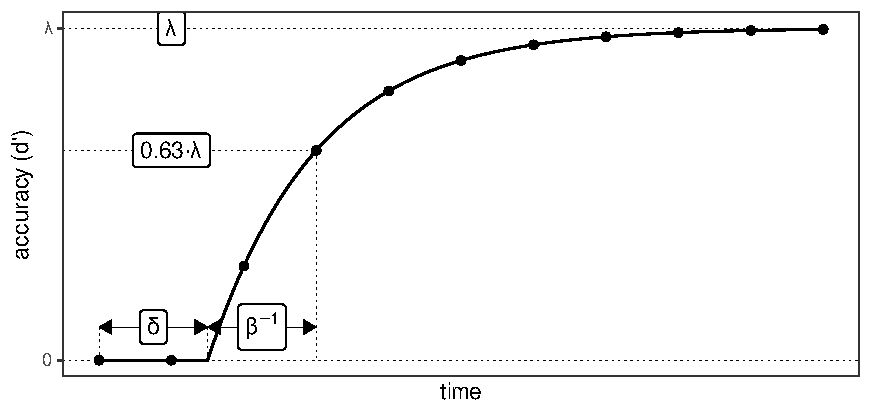
\includegraphics[width=1\columnwidth]{../figures/illustrations/illustration_satf.pdf} %[width=0.5\textwidth,height=\textheight]
\caption{\label{fig:illustrationSATF}A speed-accuracy tradeoff following equation \ref{eq:satf}. After an initial period of chance performance, accuracy begins to increase at the intercept ($\delta$). The growth rate ($\beta$) determines how quickly the function approaches the asymptotic performance ($\lambda$).
The reciprocal of the rate $\beta^{-1}$ can be interpeted as the time required for the function to reach approximately $63\%$ of the asymptote.
}
\end{figure}


Analysis of data from response signal paradigm experiments follows a variant of a stepwise model selection procedure sometimes referred to as a \textit{hierarchical model testing scheme} (e.g., \citeNP{Foraker2018}):
The aim is to select the most parsimonious of a range of models of varying complexity according to several criteria. For two-condition experiments, there are 8 candidate models. The simplest model (\(1\delta-1\beta-1\lambda\)) posits a single intercept, rate, and asymptote for both experimental conditions. The most complex model (\(2\delta-2\beta-2\lambda\)) posits separate intercepts, rates, and asymptotes for both experimental conditions. Further models of intermediate complexity that are also considered in the process are \(1\delta-1\beta-2\lambda\), \(1\delta-2\beta-1\lambda\), \(1\delta-2\beta-2\lambda\),
\(2\delta-1\beta-1\lambda\), \(2\delta-1\beta-2\lambda\), and
\(2\delta-2\beta-1\lambda\).
Each model corresponds to a particular pattern of differences between experimental conditions: Differences in asymptotes ($\lambda$) can be interpreted as differences in the success probability of the target process, while differences in rate and intercept ($\delta$ and $\beta$), jointly considered \textit{the dynamics}, can be interpreted as differences in processing speed. 

The parameters for each such model are typically estimated separately for each participant by means of numerical optimization minimizing the \textit{root mean squared error (RMSD)} of the model fit. 

For inference, \citeA{Foraker2018} recommend \textit{forward model selection} starting with the asymptote parameter $\lambda$. As illustrated in Figure \ref{fig:model_selection}A, this process works by successively comparing nested models, beginning with the simplest model \(1\delta-1\beta-1\lambda\) and \(1\delta-1\beta-2\lambda\) in order to determine whether to assume one or two asymptotes. The choice made at this point affects which models will be considered later. If there is sufficient evidence for the two-asymptote model, this means that there is a difference in asymptotes between the two experimental conditions, and only \(2\lambda\) models are considered at later stages; otherwise only \(1\lambda\) models are considered. Similarly, the choice regarding the number of intercept parameters affects which models are considered at the third stage of the forward model selection procedure, when the number of rates is determined in the example in Figure \ref{fig:model_selection}A.

An alternative is \textit{backward model selection}, illustrated in Figure \ref{fig:model_selection}B. This model selection process starts with the most complex model \(2\delta-2\beta-2\lambda\), and involves comparing it to increasingly less complex nested models. If no evidence is found for the more complex model, the simpler model is adopted.
During the stepwise selection procedure, models are compared based on (i) \textit{adjusted \(R^2\)}, which takes into account the fit and penalizes the number of parameters, and (ii) the consistency of the direction of the difference of the parameter estimates in the more complex models, as assessed by a statistical test. 
%Because we will explore the statistical power in a desi

A third alternative we will consider is non-stepwise inference based on the estimates of a \(2\delta-2\beta-2\lambda\) model. That is, we will assume that the two experimental conditions differ in a parameter if we observe a significant difference between the parameter estimates, in no particular order.
%xxx

\begin{figure}[t]
\centering
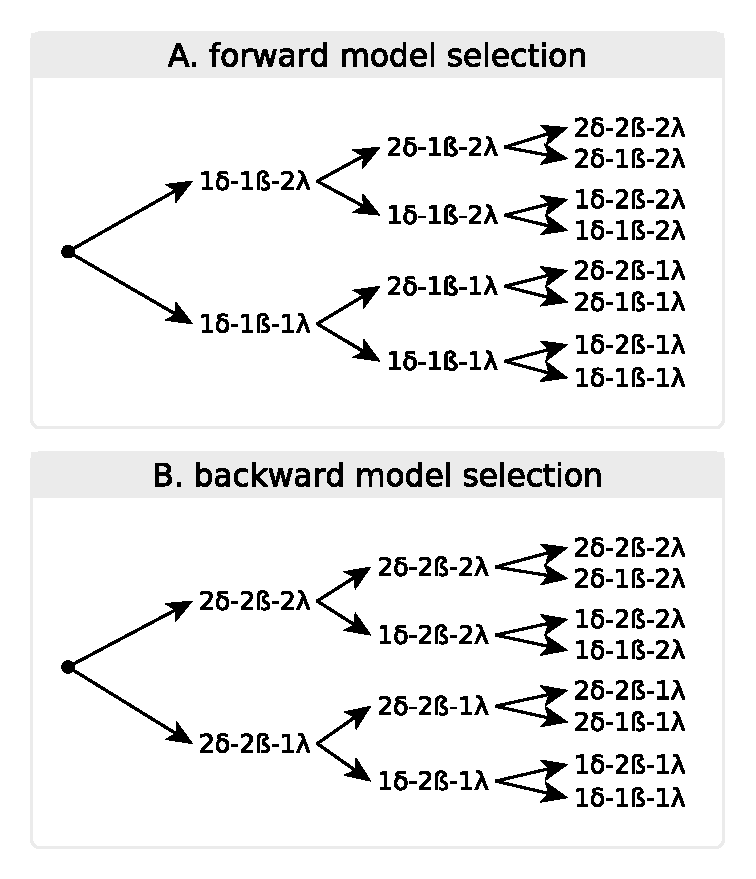
\includegraphics[width=.75\columnwidth]{../figures/illustrations/decision_algo.pdf} %[width=0.5\textwidth,height=\textheight]
\caption{\label{fig:model_selection}Illustration of the forward and backward model selection processes, in which the number of asymptotes is determined first, then the number of intercepts, and then the number of rates.}
\end{figure}

\section{Simulation Study}\label{our-simulations}

In order to determine the statistical power of the model selection methods outlined above with different sample sizes, we repeatedly simulated data for a number of different effect sizes for asymptotic accuracy and dynamics, performed model selection, and calculated the proportion of cases in which a difference with the correct sign was identified.

\subsection{Method}\label{method}

We repeatedly simulated SR-SAT and MR-SAT experiments with two experimental condition pairs (two signal conditions, and two noise conditions). Figure \ref{fig:satf_simulation} provides an overview of the process. We used parameter values which are relatively typical for sentence processing SAT experiments and assumed that the average population SATF followed equation \ref{eq:satf} with \(\delta=0.8\,sec\), \(\beta^{-1}=0.8\,sec\), \(\lambda=2.25\). We further assumed that the individual SATF parameters for each subject \(s\) (\(\lambda_S\), \(\beta^{-1}_S\), \(\delta_S\)) were log-normally distributed around the population parameters (\(SD_{\delta}=0.8\), \(SD_{\beta^{-1}}=0.8\), \(SD_{\lambda}=1.25\)). We simulated data for a range of differences between conditions in the three SATF population parameters.

%We made use of previous SAT studies  \cite<e.g.,>[among many others]{McElree2006a,McElree2006b,Foraker2007,Martin2008,VanDyke2011,Bott2012,Xiang2014} in deciding on the values for the SATF parameters, the number of participants, and the number and the lag interval of the responses. 

% all the deltas were in the the right direction, even though there was a distribution

For each combination of parameters, we simulated a participant pool of \(2,000\) participants with responses at 17 lags starting from \(0\,sec\) to \(5.6\,sec\), increasing in steps of \(0.35\,sec\). We simulated different numbers of responses per: \(20\), \(50\), and \(80\) in each of the four experimental conditions for each of the 17 lags. To simulate experiment replications, we then drew $1,000$ bootstrap samples of $10$, $20$, $30$, $40$, or $50$ participants and carried out model comparison for each bootstrap sample.  

In simulating responses, we assumed that \(P(R_{t,q}=0)\), i.e. the probability of a `noise' response in condition \(q\) at time \(t\) is given by equation \ref{eq:p_no}. We assumed that responses were equi-biased towards `signal' and `noise' responses, and that the response criterion $c$ at time $t$ was always $c_t = d_t/2$.\footnote{This assumption was made in order to obtain best-case power estimates, as a bias towards either response would increase the variance of the sampling distribution of $d'$. \cite<cf.>[for an approximation of the variance of the $d'$ sampling distribution.]{Liu2009b}}  

\vspace{-0.3cm}
\begin{equation}
\begin{split}
P(R_{t,q}=0) = \Phi(c_t-\psi_{t,q})\text{, where} \\
\psi_{t,q} =
        \begin{cases}
            d_t & \text{in signal trials} \\
            0 & \text{in noise trials}
        \end{cases}
\end{split}
\label{eq:p_no}
\end{equation}

\begin{figure*}
\centering
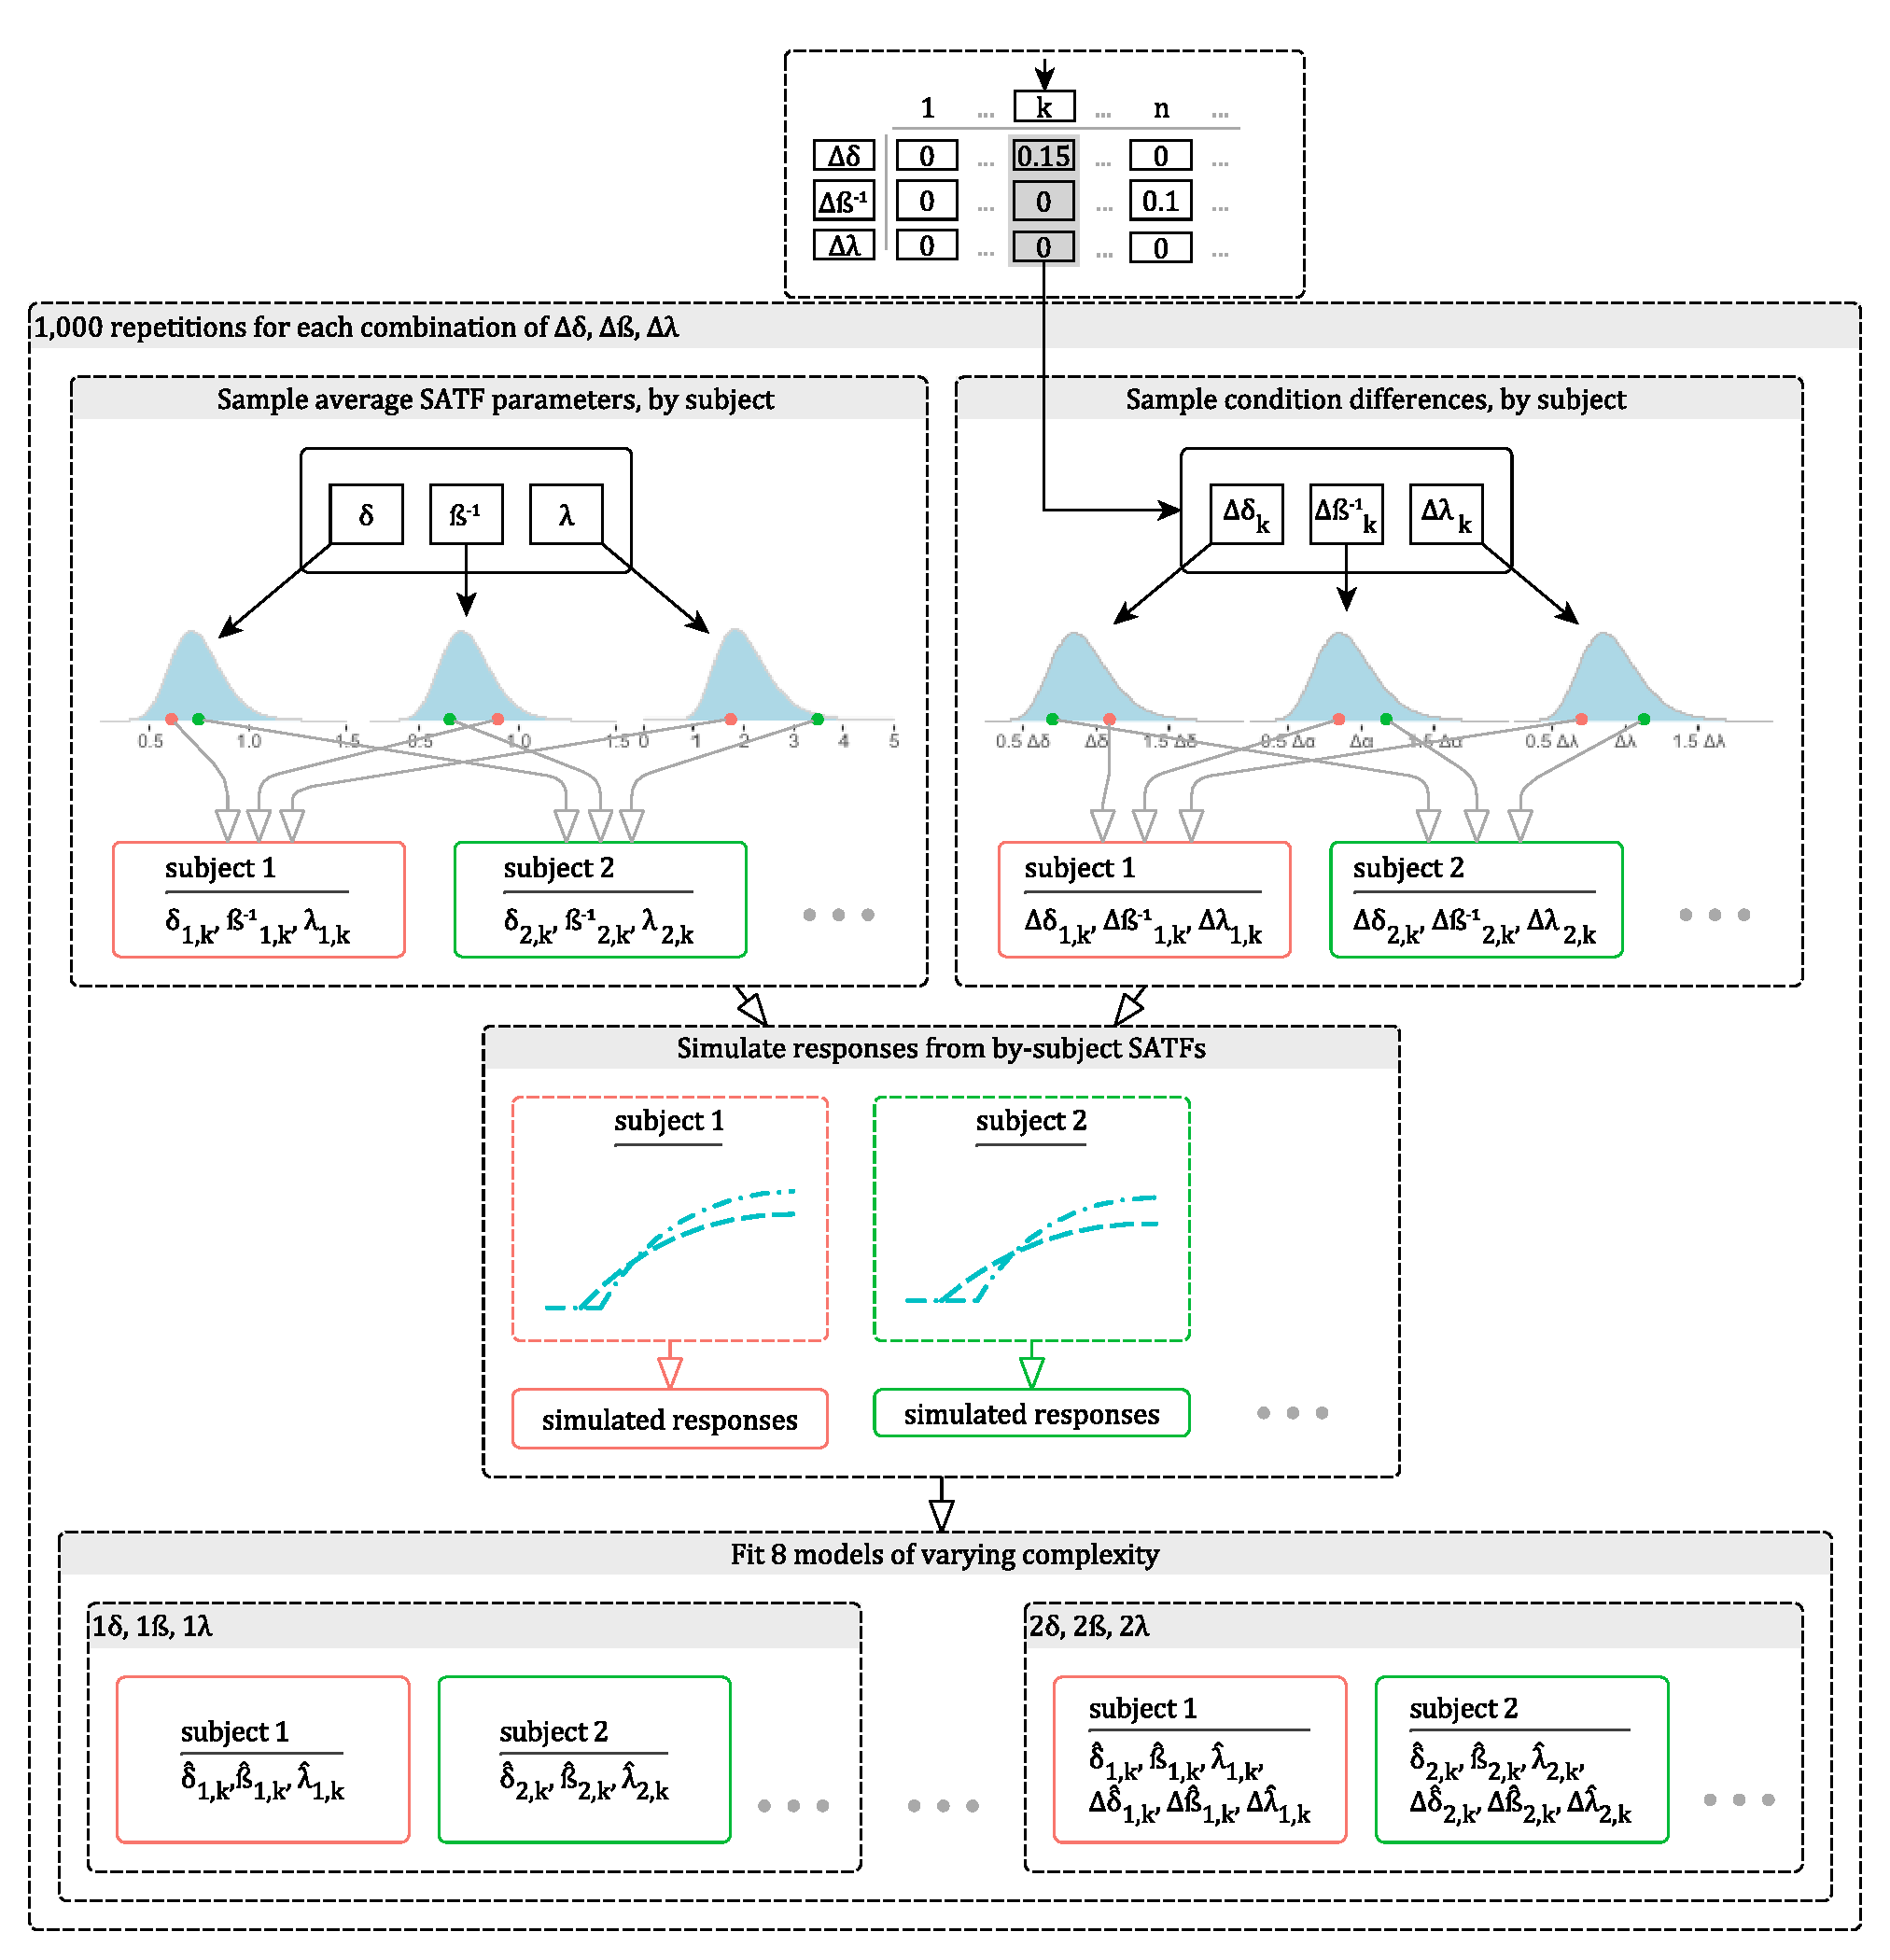
\includegraphics[width=0.9\textwidth]{../figures/illustrations/satf_simulation.pdf} %[width=0.75\textwidth,height=\textheight]
\caption{\label{fig:satf_simulation}Illustration of the simulation process: For each parameter combination for $\Delta\delta$, $\Delta\beta^{-1}$, $\Delta\lambda$, we simulated out $2,000$ participants. For each participant, we independently sampled the by-participant parameters for $\delta$, $\beta^{-1}$, $\lambda$, $\Delta\delta$, $\Delta\beta^{-1}$, and $\Delta\lambda$ from their respective distributions. We then sampled `signal'/`noise' responses for each of the 17 lags in each of the 4 conditions, computed $d'$ at each lag, for each condition pair for each simulated participant, fitted several models of varying complexity to each participants data. Next, we drew 1,000 bootstrap samples of 10, 20, 30, 40, or 50 participants each (with replacement) and carried out model comparison for each bootstrap samples. Simulations for SR-SAT and MR-SAT were carried out independently.}
\end{figure*}

Because in MR-SAT experiments, participants respond several times per trial, it stands to reason that the responses within the trial are correlated as the amount of evidence in favor of a particular response at lag \(k\) would at least partially depend on the amount of evidence available in its favor at lag \(k-1\). We modeled this serial dependence based on assumptions akin to a simple random walk model in which evidence adds up in accordance with the increase in $d'$ since the last lag: We assumed that \(\psi'_k\), the amount of evidence in favor of a `signal' response on a particular trial at lag \(k\) was the sum of \(\psi_k\), the average amount of evidence in its favor at this lag, and normally distributed serially correlated noise with mean $0$ and $\sigma=1$, as in equation \ref{eq:mr_sat}. We further assumed that a `signal' response was given when $\psi'_k > c_k$, and a `noise' response otherwise, thus accounting for serial correlation between responses.

% We further assumed that \(\psi'_k\) depended on \(\psi'_{k-1}\) as in equation \ref{eq:mr_sat}.
\begin{equation}
\begin{split}
   \psi'_k = \psi_k + \sum_{i=1}^{k} \epsilon_i/\sqrt{k} \\
            \text{where } \epsilon_i \sim N(0, 1)
\end{split}
\label{eq:mr_sat}
\end{equation}


\begin{figure*}
\centering
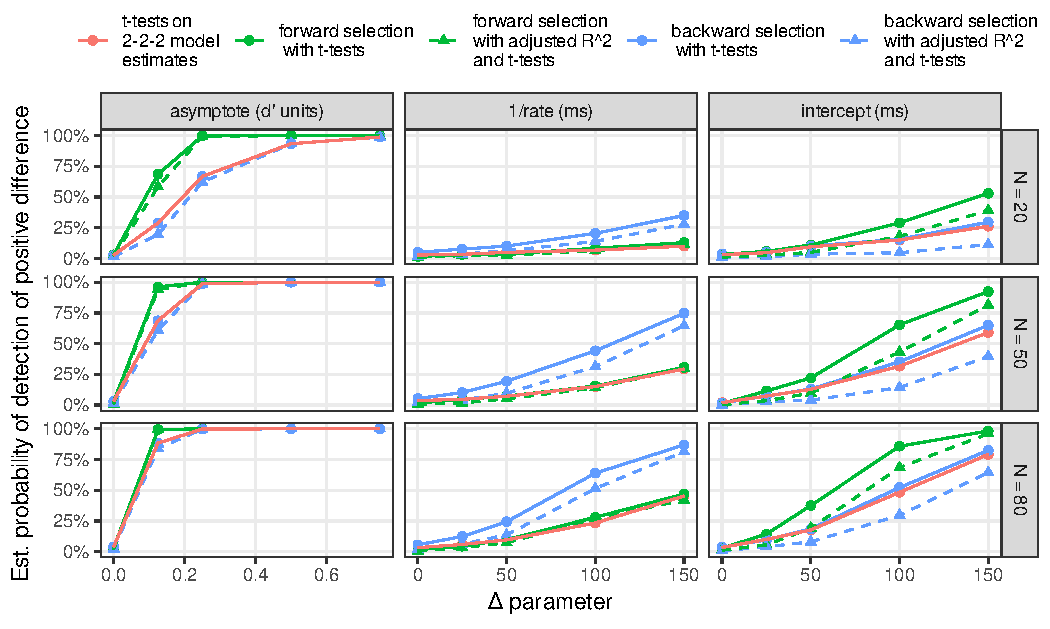
\includegraphics[width=0.94\textwidth]{../figures/results/results_sr.pdf} %[width=0.50\textwidth,height=\textheight]
\caption{\label{fig:res_sr}Simulation results for \textit{single-response SAT}. Each panel shows the simulation results for one of the three SATF parameters with a separate panel for the pooled dynamics ($\delta+\beta^{-1}$). Each cell shows the power curve estimates of a particular combination of participants (columns) and number of resposes per condition (rows). In each cell, the x-axis represents the magnitude of the population difference, while the y-axis corresponds to the proportion of simulated experiments in which a positive value for the respective difference was (correctly) detected.}

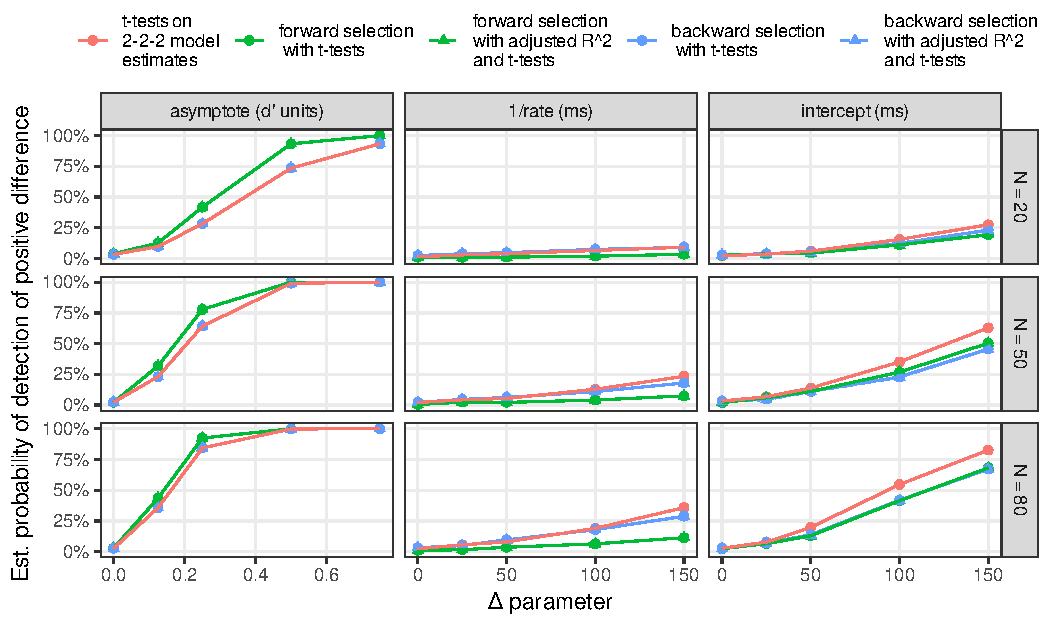
\includegraphics[width=0.94\textwidth]{../figures/results/results_mr.pdf} %[width=0.50\textwidth,height=\textheight]
\caption{\label{fig:res_mr}Simulation results for \textit{multiple-response SAT}. Layout as in figure \ref{fig:res_sr}.}
\end{figure*}

\subsection{Analysis}\label{analysis}

We used \textit{R} \cite{R-base} and the \textit{tidyverse} packages \cite{R-tidyverse} for simulation and data pre-processing, and the \textit{mrsat} R package (\citeNP{VanDyke2015}) to fit eight models of varying degrees of complexity to each simulated participant's data.

We used five different model selection procedures on each of the simulated experiments:
As a baseline analysis method, we tested for significant differences between estimates of $\hat{\delta}$, $\hat{\beta}$, $\hat{\lambda}$ in the two conditions based on $2\delta-2\beta-2\lambda$ model estimates.
Moreover, we carried out backward and forward model selection using two sets of criteria:
The first method was model selection based on the results of a t-test on the parameter difference estimates ($\hat{\Delta\delta}$, $\hat{\Delta\beta}$, $\hat{\Delta\lambda}$) of the more complex model. For example, in forward model selection as illustrated in fig. \ref{fig:model_selection}A, we selected model $1\delta-1\beta-2\lambda$ if the estimates of $\Delta\lambda$ significantly differed from $0$, or in other words: if there was a significant difference in the asymptote estimates of the two experimental conditions. Otherwise, we selected the simpler model $1\delta-1\beta-1\lambda$.
Because \citeA{Foraker2018} suggest the use of the \textit{adjusted $R^2$} metric to supplement hypothesis tests, we also tested a more conservative method, in which the more complex model was only selected if its average \textit{adjusted $R^2$} across participants was higher than that of the simpler model, in addition to the relevant parameter difference being significantly different from $0$.
%Moreover: 
%- AIC/BIC (with that group BIC approach I explain in an early draft of the SAT paper)

For the analysis of pooled dynamics $(\delta +\beta^{-1})$, we considered only $2\delta-2\beta-2\lambda$, $1\delta-1\beta-2\lambda$, $2\delta-2\beta-1\lambda$ and $1\delta-1\beta-1\lambda$ models, and based inference on the results of t-tests on the asymptote and the joint dynamics measure. 

\section{Results and Discussion}\label{results}

Figures \ref{fig:res_sr} and \ref{fig:res_mr} show the results of our simulations. In each simulation, we calculated the proportion of samples in which a positive effect was detected, because we were interested in obtaining estimates of the probability that a difference with the \textit{correct} sign is detected. As a result, the figures show estimates of \textit{(Type I error rate)/2} when there was no difference between conditions, and \textit{(Power - Type M error rate)} otherwise \cite{gelman2014beyond}. We will refer to this quantity as the detection rate. 

Importantly, since the joint dynamics measure is the sum of the intercept and the reciprocal of the rate, we could vary either to manipulate it. As a result, several detection rates are available for each value of the joint dynamics measure, depending on the contribution of the two underlying parameters. We present the maximum detection rate at each point in order to obtain optimistic detection rate estimates.
 
\subsection{SR-SAT}
The results for SR-SAT show a high overall probability of detecting a difference in asymptotes: It is  reasonably high ($>80\%$) for differences of more than $0.6$ $d'$ units, even for small sample sizes, except for the combination $10$ subjects, $20$ responses. Detection rates for the intercept parameter was rather low  ($<50\%$) for many sample sizes. Detection rates were even lower for the rate parameter, and reached more than $80\%$ only for relatively large effect sizes, and only when the sample size was high.

Interestingly, while the forward model selection methods appeared to perform better than their alternatives for the asymptote and intercept parameters, backward model selection showed the highest detection rates for the rate parameter. This discrepancy is likely due to the fact that the rate parameter is selected last in both methods. As a result, backwards model selection is less likely to attribute differences between conditions to the asymptote or to the intercept as long as the models also assume two rates. When it does not, any substantial differences between conditions have to be attributed to the rate.
As a result, backwards selection shows relatively low detection rates for asymptote and intercept differences, and relatively high detection rates for rate differences.
 
Somewhat surprisingly, the detection rates for the pooled dynamics metric $(\delta+\beta^{-1})$ did not show an improvement over detection rates for the intercept alone.  

\subsection{MR-SAT}
While the MR-SAT findings regarding the model selection method were qualitatively similar to the SR-SAT results for asymptotes and rates, the model selection method appears to matter less than for SR-SAT data.
Importantly, the MR-SAT detection rates were substantially lower across the board. This is not surprising given the fact that the responses on each trial were correlated, which is expected to increase the width of the sampling distribution and to decrease the \textit{effective sample size} \cite<e.g.,>{berger2014effective}.   
As a result, SR-SAT and MR-SAT seem to exhibit substantial differences in terms of power in detecting a difference in rates and intercepts, with remarkably low power especially for rate parameter differences of less than $50\%$ even for relatively large effect sizes such as $150\,ms$, and less than $25\%$ in most cases.  

Surprisingly, the detection rates for the pooled dynamics metric $(\delta+\beta^{-1})$ were even lower than for the intercept parameter, which was likely due to a wide sampling distribution of the rate parameter due to a lot of uncertainty. This uncertainty would increase the variance of the dynamics estimate, leading to lower detection rates.
%lot of uncertainty in the estimation of the rate parameters which are part of this metric.  

A possible concern about our findings for MR-SAT is that the exact detection rate estimates are potentially heavily dependent on the assumptions of our ad-hoc model accounting for the serial correlation between responses on a given trial. While that is correct, our results show that statistical power for MR-SAT \textit{may} be substantially lower than for SR-SAT, due to a small effective sample size. The fact that we don't know \textit{how much lower} it is, presents a major challenge in the interpretation of results from the MR-SAT methodology. 

%A possible objection to this comparison is that a fair comparison between between SR-SAT and MR-SAT should not be based on the number of responses, but on the number of trials, since multiple responses per trial are obtained in MR-SAT experiments. 




%\section{}\label{conclusion}

%\newpage
\section{Conclusions}\label{conclusions}

Our findings suggest that the statistical power for dynamics-related parameters in typical MR-SAT experiments (20 participants, with 50 responses per time lag per condition) may be relatively low for typical effect sizes in psycholinguistics ($50-100\,ms$). This is due to the fact that as a result of the serial correlation of responses on a trial, the effective sample size may be significantly lower than the nominal sample size.
As a result, the failure to find a difference in dynamics between two experimental condition pairs should be interpreted with caution.
We hope that the power can be improved and its dependence on the model selection mechanism may be remedied by simultaneous estimation of all three SATF parameters using hierarchical models such as used by \citeA{niklaus2019two} and \citeA{Pankratz2021}.
%- smart choices about positioning of measurement points
%- Use hieararchical models, like Singman et al. and Pankrantz et al.

%\section{Optional}\label{optional}
%\begin{itemize}
%\tightlist
%\item
%  Do not use this, but keep note of it:
%  Adjusted R2 is a bit of a weird metric because a unit of d' doesn't
%  really mean the same thing at d=0-1 (around the intercept), and at
%  d'=3 (around the asymptote). So the points around the asymptote, and
%  at the late increasing stage may have an undue influence. That's
%  especially problematic, since they are many.
%\end{itemize}

\bibliographystyle{apacite}

\setlength{\bibleftmargin}{.125in}
\setlength{\bibindent}{-\bibleftmargin}

\bibliography{references}


\end{document}